\documentclass{report}

\usepackage{geometry}
\geometry{a4paper,total={170mm,257mm},left=20mm,top=20mm}
\usepackage[utf8]{inputenc}
\usepackage{amsmath}
\usepackage{amsfonts}
\usepackage{amsthm}
\usepackage{amssymb}
\usepackage{bm}
\usepackage{graphicx}
\usepackage{paralist}
\usepackage[dvipsnames]{xcolor}
\usepackage{caption}
\usepackage{subcaption}
\usepackage{hyperref}
\hypersetup{urlbordercolor=ForestGreen,linkbordercolor=RoyalPurple}
\usepackage{tikz}
\usetikzlibrary{positioning}
\usetikzlibrary{intersections}
\usepackage{algpseudocode}
\usepackage{algorithm}
\usepackage{titling}
\usepackage{pgfplots}
\usepackage{fontawesome5}
 % Use the same header and libraries.
%%% Tento soubor obsahuje definice různých užitečných maker a prostředí %%%
%%% Další makra připisujte sem, ať nepřekáží v ostatních souborech.     %%%

%%% Drobné úpravy stylu

% Tato makra přesvědčují mírně ošklivým trikem LaTeX, aby hlavičky kapitol
% sázel příčetněji a nevynechával nad nimi spoustu místa. Směle ignorujte.
\makeatletter
\def\@makechapterhead#1{
  {\parindent \z@ \raggedright \normalfont
   \Huge\bfseries \thechapter. #1
   \par\nobreak
   \vskip 20\p@
}}
\def\@makeschapterhead#1{
  {\parindent \z@ \raggedright \normalfont
   \Huge\bfseries #1
   \par\nobreak
   \vskip 20\p@
}}
\makeatother

% Toto makro definuje kapitolu, která není očíslovaná, ale je uvedena v obsahu.
\def\chapwithtoc#1{
\chapter*{#1}
\addcontentsline{toc}{chapter}{#1}
}

% Trochu volnější nastavení dělení slov, než je default.
\lefthyphenmin=2
\righthyphenmin=2

% Zapne černé "slimáky" na koncích řádků, které přetekly, abychom si
% jich lépe všimli.
\overfullrule=1mm

%%% Makra pro definice, věty, tvrzení, příklady, ... (vyžaduje baliček amsthm)

\theoremstyle{plain}
\newtheorem{veta}{Věta}
\newtheorem{lemma}[veta]{Lemma}
\newtheorem{tvrz}[veta]{Tvrzení}

\theoremstyle{plain}
\newtheorem{definice}{Definice}
\newtheorem*{pozor}{Pozorování}
\newtheorem*{cvic}{Cvičení}
\newtheorem*{fakt}{Fakt}

\theoremstyle{remark}
\newtheorem*{dusl}{Důsledek}
\newtheorem*{pozn}{Poznámka}
\newtheorem*{prikl}{Příklad}

\theoremstyle{plain}
\newtheorem{thm}{Theorem}
%\newtheorem{lemma}[thm]{Lemma}
\newtheorem{claim}[thm]{Claim}

\theoremstyle{plain}
\newtheorem{defn}{Definition}
\newtheorem*{observ}{Observation}
\newtheorem*{exerc}{Exercise}
\newtheorem*{fact}{Fact}

\theoremstyle{remark}
\newtheorem*{cor}{Corollary}
\newtheorem*{rem}{Remark}
\newtheorem*{example}{Example}


%%% Prostředí pro důkazy

\newenvironment{dukaz}{
  \par\medskip\noindent
  \textit{Důkaz}.
}{
\newline
\rightline{$\qedsymbol$}
}

\newenvironment{myproof}{
	\par\medskip\noindent
	\textit{Proof}.
}{
	\newline
	\rightline{$\qedsymbol$}
}


%%% Prostředí pro sazbu kódu, případně vstupu/výstupu počítačových
%%% programů. (Vyžaduje balíček fancyvrb -- fancy verbatim.)

\DefineVerbatimEnvironment{code}{Verbatim}{fontsize=\small, frame=single}

%%% Prostor reálných, resp. přirozených čísel
\newcommand{\R}{\mathbb{R}}
\newcommand{\N}{\mathbb{N}}
\newcommand{\Z}{\mathbb{Z}}

%%% Užitečné operátory pro statistiku a pravděpodobnost
\DeclareMathOperator{\pr}{\textsf{P}}
\DeclareMathOperator{\E}{\textsf{E}\,}
\DeclareMathOperator{\var}{\textrm{var}}
\DeclareMathOperator{\sd}{\textrm{sd}}

%%% Příkaz pro transpozici vektoru/matice
\newcommand{\T}[1]{#1^\top}

%%% Vychytávky pro matematiku
\newcommand{\goto}{\rightarrow}
\newcommand{\gotop}{\stackrel{P}{\longrightarrow}}
\newcommand{\maon}[1]{o(n^{#1})}
\newcommand{\abs}[1]{\left|{#1}\right|}
\newcommand{\dint}{\int_0^\tau\!\!\int_0^\tau}
\newcommand{\isqr}[1]{\frac{1}{\sqrt{#1}}}

%%% Vychytávky pro tabulky
\newcommand{\pulrad}[1]{\raisebox{1.5ex}[0pt]{#1}}
\newcommand{\mc}[1]{\multicolumn{1}{c}{#1}}


% set up \maketitle to accept a new item
\predate{\begin{center}\placetitlepicture\large}
	\postdate{\par\end{center}}

% commands for including the picture
\newcommand{\titlepicture}[2][]{%
	\renewcommand\placetitlepicture{%
		\includegraphics[#1]{#2}\par\medskip
	}%
}
\newcommand{\placetitlepicture}{} % initialization

 % Use global macros.

\usepackage{babel}

\title{Probability and statistics 2}
\author{Filip Miháľ, Tomáš Turek}
\titlepicture[width=3in]{res/past-ii.pdf}
\date{\today}

\begin{document}
	\maketitle
	
	\INFO{This is shortened text from Probability and statistics 2. Almost all examples are omitted since this is just shortened version. Also you may find several notes of what was omitted and what is the reasoning behind that. Usually it is the lack of my time.}
	
	\tableofcontents
	\chapter{Markov chains}

\textit{"Some type of an automata, that represent probability space. It needs to have special properties."}

\begin{figure}[!h]\centering
	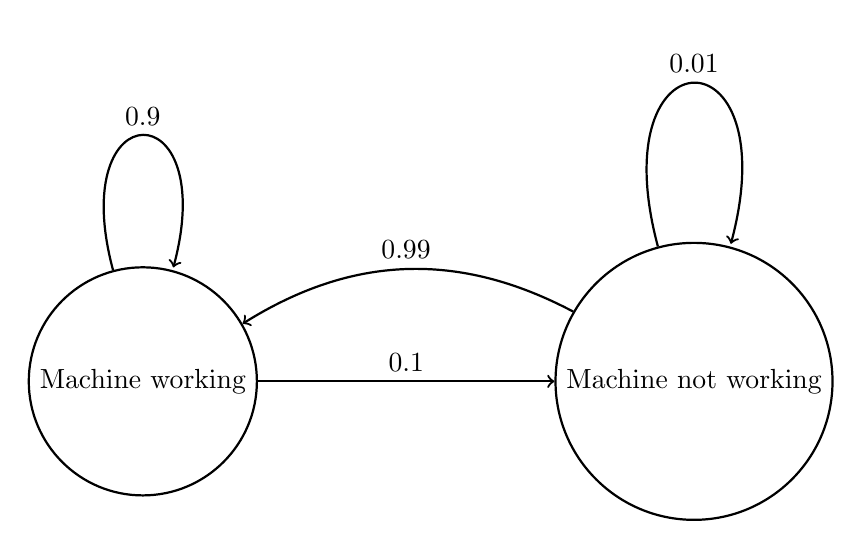
\begin{tikzpicture}[node distance={70mm}, thick, main/.style = {draw, circle}]
		\node[main] (1) {Machine working};
		\node[main] (2) [right of=1] {Machine not working};
		\path
			(1) edge [loop above] node {$0.9$} (1)
			(2) edge [loop above] node {$0.01$} (2);
		\path
			(1) edge [->] node [above] {$0.1$} (2)
			(2) edge [->] [bend right] node [above] {$0.99$} (1);
	\end{tikzpicture}
	\caption{Example of a Markov chain.}
	\label{markov-chain}
\end{figure}

\section{Model}

\begin{itemize}
	\item States: $S$ it is usually finite and sometimes only countable.
	\item sequence $X_{0}, X_{1}, X_{2}, \dots$ of random variables with values in $S$
	\item $X_{t+1}$ depends \textbf{only} on $X_{t}$
	\item $\Pr [X_{t+1} = j \vert X_{t} = i] = p_{ij}$ where $i,j \in S$
\end{itemize}

\begin{defn}
	Sequence of r.v. $X_{0},X_{1},X_{2},\dots$ is a \textbf{Markov chain} if:
	
	\begin{itemize}
		\item $\exists$ countable $S : \text{Rng } X_{t} \subset S$  $\forall t$
		\item $\forall t \in \mathbb{N}$ $\forall a_{0}, a_{1}, a_{2}, \dots , a_{t+1} \in S$
	\end{itemize}
	
	$$
	\Pr[X_{t+1} = a_{t+1} \vert X_{0} = a_{0}, X_{1} = a_{1} , \dots ,X_{t} = a_{t}] = \Pr [X_{t+1} = a_{t+1} \vert X_{t} = a_{t}]
	$$
\end{defn}

This means that Markov chain has the property of being memory-less and this probabi-\newline lity written above is called \textit{transition probability}. We can map all elements from $S$ to a number from range $1,2,\dots ,n$ and then we can build \textbf{transition matrix}.

$$
P =
\begin{pmatrix}
p_{11} & p_{12} & p_{13} & \dots \\
p_{21} & p_{22} &  \\
p_{31} &  & \ddots \\
\vdots
\end{pmatrix}
$$

Where $p_{ij}$ means going from $i$ to $j$. All $p_{ij} \geq 0$ and the sum of each row is $1$. Also we can build \textbf{transition graph} representing this Markov chain. In that graph $V = S$ and arcs exists if $(ij) : p_{ij} > 0$.

Now we look at distribution, or PMF of $X_{k} = \pi^{(k)}$ where $\pi^{(k)} = \left( \pi_{1}^{(k)}, \pi_{2}^{(k)},\pi_{3}^{(k)}, \dots \right)$ and the sum is $1$. Then we may see that $\pi_{j}^{(k)} = \Pr[X_{k} = j]$. We will be calling $\pi^{(0)}$ an \textit{initial state}.

Then we can see that $\pi^{(1)} = \pi^{(0)} P$ as multiplication by transition matrix. We can generalize this to:

$$
\pi^{(k)} = \pi^{(k-1)} P
$$

\begin{thm}
	For any \textit{MC} with transition matrix $P$ we have $\pi^{(k)} = \pi^{(0)} P^{k}$ and $\pi^{(k+1)} = \pi^{(t)} P^{k}$.
\end{thm}

\begin{proof}
	Proof will be by induction. So $\pi^{(k+1)} = \pi^{(k)} P = \pi^{(0)} P^{k} P =\pi^{(0)} P^{k+1}$.
\end{proof}

\begin{defn}
	\textbf{K-step transition} is defined as:

	$$
	\begin{array}{rcl}
	r_{ij}(k) & := & \Pr[\text{from }i \text{ to } j \text{ in } k \text{ steps}] \\
	& = & \Pr[X_{k} = j \vert X_{0} = i] \\
	& = & \Pr[X_{t+k} = j \vert X_{t} = i] \\
	r_{ij}(1) & = & p_{ij}
	\end{array}
	$$
\end{defn}

\begin{observ}
	$$
	r_{ij}(k) = \pi_{j}^{(k)} \text{ if } \pi^{0} = \left( 0, 0, \dots, 0, 1, 0 \dots, 0\right)
	$$
	
	Where $1$ is on $i$-th position. Also:
	
	$$
	\pi_{j}^{(k)} = (\pi^{0} P^{k})_{j} = \left( \left( 0, 0, \dots, 0, 1, 0 \dots, 0\right)P^{k}\right)_{j} = (P^{k})_{ij}
	$$
\end{observ}

\section{Chapman-Kologorov formula}

$$
\begin{array}{r c l}
	r_{ij}(k) & = & (P^{k})_{ij} \\
	r_{ij}(k+l) & = & \sum_{t=1}^{S} r_{it}(k)r_{tj}(l) \\
	r_{ij}(k+1) & = & \sum_{t=1}^{S} r_{it}(k) p_{tj}
\end{array}
$$

\begin{defn}
	$j$ is \textbf{accessible} from $i$ if
	
	$$
	\begin{array}{c}
		(j \in A(i), i \to j) \\
		\Updownarrow \\
		\Pr[\exists k \geq 0 : X_{k} = j \vert X_{0} = i] > 0 \\
		\Updownarrow \\
		\sum_{k=0}^{\infty} r_{ij}(k) > 0 \\
		\Updownarrow \\
		\exists \text{ a discrete path from } i \text{ to } j \\
		\text{in the transition graph}
	\end{array}
	$$
\end{defn}

\begin{defn}
	$i$ and $j$ from $S$ are \textbf{commuting states} $(i \leftrightarrow j)$ iff $i \to j$ and $j \to i$.
\end{defn}

\begin{lemma}
	$\leftrightarrow$ is an equivalence relation.
\end{lemma}

\begin{proof}
	We need to show that it satisfies reflexivity, symmetry and transitivity.
	
	\begin{enumerate}
		\item $i \leftrightarrow i$ which means $i \to i$ so $r_{ii}(0) =1$
		\item $i \leftrightarrow j$ iff $j \leftrightarrow i$ by definition
		\item $i \leftrightarrow j$ and $j \leftrightarrow t$ we want to show $i \leftrightarrow t$, but we know $i \to j \to t$ and $t \to j \to i$ so we use these paths (or just shorten them by first intersection).
	\end{enumerate}
\end{proof}

\begin{defn}
	An \textbf{equivalence class} in a Markov chain is a set of states that are commuting with each other. The set is maximal with its property. In other words, no additional state from $S$ can be included in the set without breaking the commuting property.
\end{defn}

\begin{defn}
	\textit{MC} is called \textbf{irreducible} if $\leftrightarrow$ has just $1$ equivalence class. This is equivalent to that $\forall ij : i \leftrightarrow j$.
	
	Or by graph theory we can say that the transition graph is strongly connected and when we compress these classes we get DAG.
\end{defn}

\begin{defn}
	$i \in S$ is called \textbf{recurrent} if $\forall j \in A(i) : i \in A(j)$ and \textbf{transient} otherwise.
\end{defn}

\begin{thm}
	$i \in S$ we define $f_{ii} = \Pr[\exists t \geq 1 : X_{t} =i \vert X_{0} = i]$ or by words "probability of going back to $i$". Then:
	
	\begin{itemize}
		\item $i$ is recurrent iff $f_{ii} = 1$
		\item $i$ is transient iff $f_{ii} < 1$
	\end{itemize}
\end{thm}

\begin{proof}
	$i$ is transient iff $\exists j \in A(i) : i \notin A(j)$. Starting with $X_{0} = i$ the probability $\exists t \geq 1 : X_{t} = j$ is $p > 0$ and $\Pr[\text{going to } i \text{ from } j] = 0 \Rightarrow f_{ii} \leq 1 - p$. And if $i$ is recurrent then $f_{ii} = 1$.
\end{proof}

\begin{defn}
	$i \in S$ we define $V_{i}$ as number of visits to $i$ or written as $|\{t : X_{t} = i\}|$
	
	$V_{i} \in \mathbb{N} \cup \{\infty\}$ so it is a random variable defined by $X_{0}, X_{1}, \dots$
\end{defn}

\begin{thm}
	$i$ is recurrent $\Rightarrow \Pr[V_{i} = \infty | X_{0} = i] = 1$
	
	$i$ is transient $\Rightarrow (V_{i} \vert X_{0}= i) \sim \text{Geom}(1 - f_{ii})$, where $(1-f_{ii})$ is called as \textit{escape probability}.
\end{thm}

\section{Steady state}

\begin{defn}
	Let $\pi$ be a distribution on $S$ such that $\left( \pi_{1} + \pi_{2} + \dots + \pi_{S} = 1, \pi_{i} > 0\right)$. Then $\pi$ is \textbf{stationary} distribution if $\pi P = \pi$. Or can be written as \newline $\left[ \pi = (\pi_{1}, \pi_{2}, \dots) \vert \forall j \pi_{j} = \sum_{i \in S} \pi_{i} p_{ij}\right]$ for \textit{MC} with transition matrix $P$.
\end{defn}

\begin{observ}
	If $\pi^{(0)} = \pi$ and $\pi$ is stationary then $\pi^{(1)} = \pi$ and $\forall k : \pi^{(k)} = \pi$.
\end{observ}

\begin{defn}
	$s \in S$ is \textbf{periodic} if $\exists \Delta \geq 2$ integer such that $\Pr[X_{t} = s \vert X_{0} = s] > 0 \Rightarrow \Delta \vert t$. \textit{MC} is periodic if all its states are periodic, otherwise it is \textit{aperiodic}.
\end{defn}

\begin{thm}
	$(X_{t})_{t = 0}^{\infty}$ is a \textit{MC} that is \textit{irreducible}, \textit{aperiodic} and $|S| < \infty$. Then $\exists \pi$ that is a stationary distribution and $\forall j \forall i \lim_{k\to\infty}r_{ij}(k) = \pi_{j}$, $\pi$ is a unique solution to
	
	$$
	\pi P = \pi
	$$
	
	$$
	\pi \mathbf{1} = 1
	% vector of 1s
	% TODO: I think this is wrong. Pi is a probability distribution, so if pi_j is 1, then all other indexes must be 0.
	$$
\end{thm}

\section{Absorption probability}

\begin{defn}
	Absorption states are such states, that the probability of staying in the same state is $1$. Or it is $\{s \in S : p_{ss} = 1\}$.
\end{defn}



\begin{lemma}[Probability of Absorption]
	Assume a \textit{MC} with absorbing state $0$ (and some move). Put
	
	$$
	a_{i} = \Pr[\exists t : X_{t} = 0 \vert X_{0} = i] \text{ for } i \in S
	$$
	
	Then $(a_{i})$ are the unique solution to:
	
	$$
	\begin{array}{rcll}
		a_{0} & = & 1 \\
		a_{i} & = & 0 &\text{ if } i \neq 0 \text{ and absorbing} \\
		a_{i} & = & \sum_{j \in S} p_{ij} a_{j} & \text{ for } i \text{ not absorbing}
	\end{array}
	$$
\end{lemma}

\begin{proof}
	$a_{0} = 1$ and $a_{i} = 0$ if $i \neq 0$ and absorbing is easy observation. Lets assume $i$ is not absorbing then
	
	$$
	\begin{array}{r c l}
		a_{i} & = & \Pr[\exists t : X_{t} = 0 \vert X_{0} = i] = \\
		& = & \sum_{j \in S} \Pr[X_{1} = j \vert X_{0} = i] \cdot \Pr[\exists t : X_{t} = 0 \vert X_{0} = i, X_{1} = j] = \\
		& = & \sum_{j \in S} p_{ij} \Pr[\exists t : X_{t} = 0 \vert X_{0} = j] = \\
		& = & \sum_{j \in S} p_{ij} a_{j} \\
	\end{array}
	$$
\end{proof}

\section{Mean time to absorption}

$A \subseteq S$ is set of all absorption states. $T = \min \{ t \geq 0 \vert X_{t} \in A\}$ is \textit{absorption time} and random variable. Then we define $\mu_{i} = \mathbb{E} [T \vert X_{0} = i]$.

\begin{thm}
	$(\mu_{i})_{i \in S}$ is the unique solution to:
	
	$$
	\begin{array}{rrcl}
		\text{if } i \in A & \mu_{i} & = & 0 \\
		\text{if } i \notin A & \mu_{i} & = &1 + \sum_{j \in S} p_{ij}\mu_{j}
	\end{array}
	$$
\end{thm}

\section{SAT}

Problem where there is given a Boolean formula and we have to say if it is satisfiable.

\subsection{2-SAT (polynomial)}

Special case of \textit{SAT} where all clauses have at most $2$ literals.

\subsubsection{Algorithm for 2-SAT}

\begin{enumerate}
	\item Start with any assignment $(x_{1} = x_{2} = \dots = x_{n} = F)$
	\item Repeat up to $2mn^{2}$ times ($n$ is the number of variables and $m$ is an arbitrary parameter)
	\begin{itemize}
		\item if $\varphi$ is satisfiable return "YES"
		\item otherwise, choose any clause that is not satisfied and randomly change one of its variables $(\ast)$
	\end{itemize}
	\item Return "NO"
\end{enumerate}

$Pr[\text{incorrectly saying no}]  \leq \frac{1}{2m}$ which can be proved by Markov inequality.

$Pr[\text{incorrectly saying no}]  \leq \frac{1}{2^m}$ using iterative Markov inequality.

\subsection{3-SAT}

\subsubsection{Algortihm for 3-SAT}

\begin{itemize}
	\item Repeat for $\leq m$ times
	\begin{itemize}
		\item Repeat for $\leq 3^{n/2}$ times
		\begin{itemize}
			\item randomly initialize the variables
			\item if $\varphi$ is satisfiable return "YES"
			\item otherwise, choose any clause that is not satisfied and randomly change one of its variables
		\end{itemize}
	\end{itemize}
\end{itemize}

Running time of this algortihm is exponential in $n$.

$P[\text{failure}] \leq \frac{1}{2^m}$

By using a better algorithm we can get the exponential part to be $\frac{4^n}{3}$.

The idea behind these algorithms is that we are using a \textit{random walk} on the space of all possible assignments. This is a \textit{Markov chain}. So we can easily calculate the probability of getting to the absorbing state and the mean time to get there.

	\chapter{Bayesian statistics}

\section{What is probability?}

We may look at probability from different angles.

\begin{enumerate}
	\item Math concepts.
	\begin{itemize}
		\item axioms, examples $\frac{\# \text{good}}{\#\text{all}}$, theorems ...
		\item interesting/useful probabilistic method as "to show $A \neq 0$ we show $\Pr[A] >0$", lower bounds for Ramsey number
	\end{itemize}
	\item Description of real world. Question: \textit{Does Nature play dice?}
	\begin{itemize}
		\item YES, if quantum theory is right so called \textit{true randomness}
		\item imprecise measurements so called \textit{pseudo randomness}
	\end{itemize}
\end{enumerate}

Then we we have two possible approaches.

\begin{enumerate}
	\item \textbf{Frequntist's approach} $\frac{\text{\# good}}{\text{\# all}}$
	\item \textbf{Bayesian approach} as subjective probability, so we are counting with all possible universes and what is the probability this will happen in our universe.
\end{enumerate}

\section{Bayesian statistics}

\begin{enumerate}
	\item $\Theta$ is random variable describing some quantity of interest
	\item $X = (X_{1}, \dots, X_{n})$ measurements
\end{enumerate}

\begin{rem}
	In Frequentist's approach $\Theta$ does not exist we have $\vartheta$ as unknown fixed \newline parameter.
\end{rem}

\begin{table}\centering
	\begin{tabular}{| c | c | c |}
		variable & PMF          & PDF          \\
		\hline
		1 & $p_{\Theta}$ & $f_{\Theta}$ \\
		2 & $p_{X}$ & $f_{X}$ \\
	\end{tabular}
\end{table}

\subsection{Bayes theorem}

$$
\Pr[B \vert A] = \frac{\Pr[B] \Pr[A \vert B]}{\Pr[A]}
$$

Where $\Pr[A], \Pr[B] > 0$. We will consider $B$ as $\Theta = \vartheta$ and $A$ as measurements $X = x$. Now we get:

$$
\Pr[\Theta = \vartheta \vert X = x] = \frac{\Pr[\Theta = \vartheta] \Pr[X = x \vert \Theta = \vartheta]}{\Pr[X = x]}
$$

Where $\Pr[\Theta = \vartheta \vert X = x]$ is called \textbf{posterior} and it is the probability after some measurements. $\Pr[\Theta = \vartheta]$ is called \textbf{prior} as an probability and $\Pr[X = x \vert \Theta = \vartheta]$ is our current model of the world (\textit{likelihood}).

\subsection{Bayes theorem using PMF}

$$
p_{\Theta\vert X} (\vartheta \vert x) = \frac{p_{\Theta}(\vartheta) p_{X\vert\Theta}(x \vert \vartheta)}{\sum_{\vartheta'} p_{\Theta}(\vartheta')p_{X\vert\Theta}(x \vert \vartheta')} = c p_{\Theta}(\vartheta) p_{X \vert \Theta}(x \vert \vartheta)
$$

For some constant $c$.

\section{What do we want?}

\begin{enumerate}
	\item Point estimate for $\Theta$.
	\item Interval estimate for $\Theta$.
	\item Hypothesis testing.
\end{enumerate}

For \textit{interval estimate} we have given $X$ and want to find $[a,b]$ as $(a = a(X), b = b(X))$. $\Pr[a(x) < \Theta < b(X) \vert X = x] \geq 1 - \alpha$. Perhaps $\Pr[\Theta < a(x) \vert X =x ] = \frac{\alpha}{2}$ and $\Pr[\Theta > b(x) \vert X =x ] = \frac{\alpha}{2}$.

For \textit{point estimate} we have two approaches.

\subsection{1) MAP as for maximum aposteriori probability}

$$
\hat{\vartheta} = \arg\max_{\vartheta} p_{\Theta \vert X} (\vartheta \vert x)
$$

If $X = x$ what is the most likely value?

\subsection{2) LMS as for least mean square}

$$
\begin{array}{rcl}
\hat{\vartheta} & = & \arg\min_{\vartheta} \mathbb{E}[(\Theta - \vartheta)^{2} \vert X = x] \\
& = & \arg\min_{\vartheta} \mathbb{E}[\Theta \vert X = x]
\end{array}
$$

\section{Naive Bayes}

By the Bayesian statistics we get for $X_{1}$:

$$
p_{\Theta\vert X_{1}} (\vartheta \vert x_{1}) = \frac{p_{\Theta}(\vartheta) p_{X_{1} \vert\Theta}(x_{1} \vert \vartheta)}{\sum_{\vartheta'} p_{\Theta}(\vartheta')p_{X_{1}\vert\Theta}(x_{1} \vert \vartheta')}
$$

But what if we have $n$ measurements to consider. Then we have $\Pr[\Theta = \vartheta \vert X_{1} = x_{1}, X_{2} = x_{2}, \dots]$ which can be computed by naive Bayes as:

$$
= \frac{p_{\Theta}(\vartheta) \prod_{i=1}^{n}p_{X_{i}\vert \Theta} (x_{i} \vert \vartheta)}{\sum_{\vartheta'} p_{\Theta}(\vartheta')\prod_{i=1}^{n}p_{X_{i}\vert \Theta} (x_{i} \vert \vartheta')}
$$

Also $p_{X \vert \Theta}(x_{i}, \dots, x_{1} \vert \Theta = \vartheta)$ is \textit{joint PMF} and we assume conditional independence.

\section{Bayes theorem using PDF}

As for PMF we have Bayesian statistics for PDF.

$$
f_{\Theta \vert X}(\vartheta \vert x) = \frac{f_{\Theta}(\vartheta) f_{X \vert \Theta}(x \vert \vartheta)}{\int_{-\infty}^{\infty} f_{\Theta}(\vartheta') f_{X \vert \Theta} (x \vert \vartheta') \text{ d} \vartheta'}
$$

\section{Beta distribution}

To see some nice properties of Bayesian theorem we will look into one new distribution. We will have $\alpha, \beta \geq 1$ and $\vartheta \in [0,1]$. Then

$$
f_{\Theta} (\vartheta) = \frac{\vartheta^{\alpha - 1} (1-\vartheta)^{\beta - 1}}{B (\alpha,\beta)}
$$

Where $B(\alpha, \beta)$ is called \textbf{beta function} and for all $\alpha, \beta$ it is a constant. For example the beta function for $B(1,1)$ is equal to $1$ from $[0,1]$ and $0$ otherwise. And $B(1,2) = \frac{1}{2}$. It serves as a normalizing constant for the beta distribution.

Firstly the maximum is at $\frac{\alpha -1}{\alpha + \beta - 2}$ which is the \textbf{mode} (\textit{cz: modus}).

Secondly:

$$
B(\alpha, \beta) = \frac{(\alpha - 1)! (\beta - 1)!}{(\alpha+\beta-2)!} = \frac{1}{\binom{\alpha + \beta - 2}{\alpha -1}}
$$

Lastly $\mathbb{E} [\Theta] = \frac{\alpha}{\alpha + \beta}$ which is the \textbf{mean}.

Now we will look into the Bayesian theorem using Beta distribution as a prior and Binomial distribution as a likelihood.

$$
p_{X \vert \Theta}(k \vert \vartheta) = \binom{n}{k} \vartheta^{k} (1-\vartheta)^{n-k}
$$

$$
f_{\Theta \vert X}(\vartheta \vert x) = c_{1} \vartheta^{\alpha - 1}(1 - \vartheta)^{\beta - 1} \cdot c_{2} \vartheta^{x} (1- \beta)^{1-x} \cdot c_{3} =
$$

Where $c_{1},c_{2},c_{3}$ do not depend on $\vartheta$ and are some constants.

$$
= c_{4} \vartheta^{\alpha + k -1}(1 - \vartheta)^{\beta + n - k -1}
$$

And that is some other Beta distribution with $\alpha' = \alpha + x$ and $\beta' = \beta + n - x$. And also we have these point estimates:

\begin{enumerate}
	\item MAP $\hat{\vartheta} = \frac{x}{n}$ which is same as likelihood.
	\item LMS $\hat{\vartheta} = \mathbb{E}(\Theta \vert X = x) = \frac{x+1}{n+2}$
\end{enumerate}

\section{Normal random variable}

Also we can look at Bayesian theorem with normal variables. \textit{Note: This doesn't seem so interesting and useful, since it is only computation and nothing else.}

% TODO: have a look at this if you have any time left.

\section{Conditional expectation}

Firstly we will remind how expectation is defined. $\mathbb{E}[Y] = \sum_{y \in \text{Img}(Y)} y \Pr[Y = y]$ if $Y$ is discrete or $= \int_{-\infty}^{\infty} y f_{Y}(y) \text{ d}y$ if $y$ is continuous. Now we will show how conditional expectation is defined.

$$
\begin{array}{rcl}
\mathbb{E}[Y \vert A] & = & \sum_{y \in \text{Img}(Y)}y \Pr[Y = y \vert A] \\ \\
& = & \int_{-\infty}^{\infty} y f_{Y \vert A}(y) \text{ d}y
\end{array}
$$

Now if we have $X,Y$ discrete random variables and $x \in \mathbb{R}$, then:

$$
\mathbb{E}[Y \vert X = x] =: g(x)
$$

So $g$ is a function $\mathbb{R} \to \mathbb{R}$. Then

$$
\mathbb{E} [Y \vert X] =: g(X)
$$

So we have two functions $\Omega \to^{X} \mathbb{R} \to^{g} \mathbb{R}$. Now we will show one property which is called \textbf{Law of Iterated Expectation}.

$$
\mathbb{E}[\mathbb{E}[Y \vert X]] =^{\text{DEF}} \mathbb{E}[g(X)] =^{\text{LOTUS}} \sum_{x \in \text{Img}(X)}g(x) \Pr[X = x] =
$$

$$
=^{\text{DEF}} \sum_{x \in \text{Img}(X)}\Pr[X=x] \mathbb{E} [Y \vert X =x] = \mathbb{E}[Y]
$$

Where the last equivalence is by the Law of total Expectation. So by this we get $\mathbb{E}[\mathbb{E}[Y \vert X]] = \mathbb{E}[Y]$ if $\mathbb{E}[Y] < \infty$.

Now, we will use a similar approach to find an alternative definition of variance.

Let $Y = \hat{Y} - \tilde{Y}$ where $\hat{Y}$ and $\tilde{Y}$ are statistically independent and $var(\tilde{Y}) = \mathbb{E}[\tilde{Y}^2]$

$$
var(Y) = var(\hat{Y}) + var(\tilde{Y}) - 2cov(\hat{Y}, \tilde{Y})
$$

From the property of the statistical independence we get $cov(\hat{Y}, \tilde{Y}) = 0$.

$$
\mathbb{E} [(Y - E[Y\vert X])^2 \vert X] = var[Y \vert X] =: h(X)
$$

\section{Law of iterated variance}

$$
\text{var} [Y] = \mathbb{E}[\text{var}[Y \vert X]] + \text{var}[\mathbb{E}[Y \vert X]]
$$

Or it is called an \textbf{Eve's rule} (\textit{as E for expected value and V for variance}). We may simulate it by saying that the first part of the sum is expected value of variance within one group and the second part is inter group variance. \textit{This is also partly from the example that was sadly omitted.}

Next we can show that Least Mean Square is iff condition expectation. That is for given $Y$ what is the value of $y$ that minimizes $\mathbb{E}[Y - y]^{2}$?

$$
\mathbb{E}[Y - y]^{2} = \mathbb{E}[Y^{2}] - 2y\mathbb{E}[Y] + y^{2} = f(y)
$$

$$
f'(y) = - 2 \mathbb{E}[Y] + 2y = 0 \Rightarrow y = \mathbb{E}[Y]
$$

Now we want for all $x$ find $y = y(x)$ such that $\mathbb{E}[(Y - y(x))^{2} \vert X = x]$ is minimized. We can show by similar calculation that $y(x) = \mathbb{E}[Y \vert X =x ]$. And our best (in the LMS sense) estimation is $\hat{Y} = \mathbb{E} [Y \vert X]$.

	\chapter{Stochastic processes}

Stochastic process is a sequence of random variables $X_{1}, X_{2}, X_{3}, \dots$. We will show that there exist many of them.

\begin{itemize}
	\item Markov chain (+ extra condition)
	\item Wiener process
	\begin{itemize}
		\item Browner motion
		\item Stock prices
		\item Limit version of RN
	\end{itemize}
	\item \textbf{Arrival times} or alternatively \textbf{waiting for success}.
\end{itemize}

We will be looking at the last type of the processes.

\section{Bernoulli process (denoted as $\text{Bp}(p)$)}

That is we have $X_{1}, X_{2}, \dots$ iid and each one of them is $X_{i} \sim \text{Ber}(p)$ so with probability $p$ it is $1$ and $0$ with probability $1-p$.

\begin{observ}
	\begin{itemize}
		\item $X_{n}, X_{n+1}, \dots$ is also $\text{Bp}(p)$
		\item $X_{N}, X_{N+1}, \dots$ is also $\text{Bp}(p)$, with $N$ a random variable dependent only on the past
	\end{itemize}
\end{observ}

Then we will define $T =\min \{t : X_{t} = 1\}$ or by words the time of the first success / arrival. And we can easily see that $T \sim \text{Geom}(p)$ so $\mathbb{E}[T] = \frac{1}{p}$ and $\text{var} [T] = \frac{1-p}{p^{2}}$.

Now we will try to generalize this by $T_{k}$ as the time of the $k$-th arrival. So $T_{1} = T$. Or written as $T_{k} = \min \{t : X_{1} + X_{2} + \dots + X_{t} = k\}$.

Other interesting variable is the $k$-th waiting time (inter arrival) and it will be denoted as $L_{k}$. To describe this variable it is the time between $k-1$ arrival and $k$-th arrival. Then it follows

$$
L_{k} = T_{k} - T_{k-1} \text{ when we put } T_{0} = 0
$$

$$
L_{k} \sim L_{1} = T \Rightarrow L_{k} \sim \text{Geom}(p)
$$

And all $L_{i}$ are independent. From the other way we can define $T_{k}$ as the sum $\sum_{i=1}^{k} = L_{i}$. So we can then get expected value and variance.

$$
\mathbb{E}[T_{k}] = \mathbb{E}[L_{1}] + \mathbb{E}[L_{2}] + \dots + \mathbb{E}[L_{k}] = \frac{k}{p}
$$

$$
\text{var}[T_{k}] = \text{var}[L_{1}] + \text{var}[L_{2}] + \dots + \text{var}[L_{k}] = k \cdot \frac{1-p}{p^{2}}
$$

How could we compute $\Pr[T_{k} = t] = ?$ Easily we can compute this by convolution formula $\binom{t-1}{k-1} p^{k}(1-p)^{t-k}$.

Lastly we define $N_{t}$ as the sum $X_{1} + X_{2} + \dots + X_{t}$ which is the number of successes till the time $t$. And $N_{t} \sim \text{Bin}(t,p)$. So $\mathbb{E}[N_{t}] = tp$ and $\text{var}[N_{t}] = tp(1-p)$.

\subsection{Alternative definition}

We can define Bernoulli process by different definition. First we will define $L_{1}, L_{2}, \dots$ as iid $\sim \text{Geom}(p)$ and then $T_{k} = \sum_{i=1}^{k} L_{i}$. And $X_{i}$ is $1$ if $T_{k} = i$ for some $k$ or $0$ otherwise. Then $(X_{i})_{i}$ is $\text{Bp}(p)$.

\subsection{Merging of Bernoulli process}

We will have two processes which are independent.

$$
\begin{array}{rl}
X_{1}, X_{2}, X_{3}, \dots & \text{Bp}(p) \\
Y_{1}, Y_{2}, Y_{3}, \dots & \text{Bp}(q)
\end{array}
$$

Then the merge is $Z_{i} = X_{i} \text{ or } Y_{i}$. Properly it is

$$
\begin{array}{rl}
Z_{1}, Z_{2}, Z_{3}, \dots & \text{Bp}(p + q - pq) = \text{Bp}(1 - (1-p)(1-q))
\end{array}
$$

\subsection{Splitting Bernoulli process}

We can also split one Bernoulli process. Firstly we got

$$
\begin{array}{rl}
Z_{1}, Z_{2}, Z_{3}\dots & \text{Bp}(r)
\end{array}
$$

If $Z_{i}=1$ then $X_{i} = 1$ with probability $\alpha$ and $0$ with probability $(1 - \alpha)$ and if $Z_{i} = 0$ then $X_{i}=0$. By this construction we get new Bernoulli process.

$$
\begin{array}{rl}
X_{1}, X_{2}, X_{3}, \dots & \text{Bp}(\alpha r)
\end{array}
$$

\section{Poisson process (denoted as $\text{Pp}(\lambda)$)}

As we defined Bernoulli process we also can define Poisson process which can be described as a continuous approximation of $\text{Bp}(p)$. Now the arrival times are real numbers.

\begin{defn}
	\begin{enumerate}
		\item For any interval of length $\tau$ probability of $k$ arrivals is the same. Denoted as $P(k, \tau)$.
		\item Number of arrivals in $[a,b]$ is independent of number in $[0, a)$.
		\item $P(0, \tau) = 1 - \lambda \tau + o(1)$, $P(1, \tau) = \lambda \tau + o(1)$, $P(k, \tau) = o(1)$. for $k \geq 2$ where $o(1)$ is something that goes to zero
	\end{enumerate}
\end{defn}

% TODO: What is the small o??

Then the sequence $T_{1}. T_{2}, T_{3}, \dots$ is $\text{Pp}(\lambda)$ where Ts are the arrival times.

% $Pr[N_t = k] = P(k, t) = $

As in Bernoulli process we have $T_{k}$ as the time of $k$-th arrival. Then $N_{T}$ is the number of arrivals in $[0,t]$ and $N_{T} \sim \text{Pois}(\lambda t)$ so $P(k, t) = e^{-\lambda t} \frac{(\lambda t)^{k}}{k!}$.

We can show that by the following approximation:

$$
\begin{array}{c}
	Pr[N_t = k] = P(k,t) \implies P(1, \frac{t}{l}) = \frac{\lambda t}{l} + o(1) \\
	Pr[N_t = k] = P(k, t) \approx P[\text{there are K small intervals that has 1 arrival}] = \\
	= Pr[Bin(l, \frac{\lambda t}{l}) = k] \newline \implies lim_{l \to \infty} Bin(l, \frac{\lambda t}{l}) \to Pois(\lambda  t)
\end{array}
$$

Then again $L_{k} = T_{k} - T_{k-1}$ so $\Pr[L_{k} \geq t] = \Pr[\text{no arrival in }[T_{k-1}, T_{k-1}+t]]$ and that is equal to $P(0,t) = e^{-\lambda t}$. Next $\Pr[L_{k} \leq t] = 1 - e^{-\lambda t} \Rightarrow L_{k} \sim \text{Exp}(\lambda)$.

\subsection{Alternative description}

As in Bernoulli process we can define Poisson process the other way around. We start with sequence of iid $L_{1}, L_{2}, \dots \sim \text{Exp}(\lambda)$. Then $T_{k}$ is the sum $T_{k} = \sum_{i=1}^{k} L_{i}$. And we also get the same $N_{t}$.

\begin{thm}
	This also defines $\text{Pp}(\lambda)$. In other words it satisfies all of the three properties.
\end{thm}

Again as in Bp we can see that expected value of $T_{k}$ and variance is the sum of expected values (resp. variances) of $L_{i}$ which are $\frac{1}{\lambda}$ (resp. $\frac{1}{\lambda^{2}}$). By convolution we get that

$$
f_{T_{k}} (t) = \frac{\lambda^{k} t^{k-1}e^{-\lambda t}}{(k-1)!}
$$

\subsection{Splitting of Pp}

We have a $\text{Pp}(\lambda)$ and each one is split (1 or 0) with probability $p$ (resp. $1-p$). And then we get two processes $\text{Pp}(p \lambda)$ and $\text{Pp}((1-p) \lambda)$ and these are independent. Two new processes have still the same properties but with new $\lambda'$. To properly show that this holds we need to show all the properties from the definition.

% TODO

$$
Pr[T_1 > t] = Pr[T>t \ \&  \ T' > t] =  \dots
$$

\begin{rem}
	Proving independence is quite cumbersome. The proof is based on an example from the lecture.
\end{rem}

\subsection{Merging of Pp}

If we have two processes $\text{Pp}(\lambda)$ and $\text{Pp}(\lambda')$ we can merge these to get $\text{Pp}(\lambda + \lambda')$. Again to properly show that this holds we must show that the $\min$ of two $\text{Exp}$ distributions is again $\text{Exp}$ distribution with the sum. Which is quite easy since they are independent, then we get the product of exponent functions which is the same as the sum of their exponents.

What if we look at the $\Pr[T - t > s \vert T > t]$ which by definition is $\frac{\Pr[T > s+t \land T > t]}{\Pr [T > t]}$ and that is equal to $\frac{e^{-\lambda (s+t)}}{e^{-\lambda t}} e^{-\lambda s}$ and we get the property that the Poisson process is \textbf{memory-less} so it doesn't matter when we will start measuring our data.

	\chapter{Balls \& Bins}

This model is if we have $m$ balls and $n$ bins and for each ball we put it independently at random to one bin, where each bin has the same probability.

One well known problem is \textit{Birthday paradox} where we have $k$ people as balls and $365$ days as bins. Then we are asking what is the probability that one bin has at least 2 balls.

$$
Pr[\text{at least 2 balls in one bin}] = 1 - Pr[\text{max 1 ball in one bin}] =
$$

$$
= 1 - \prod_{i=1}^{m-1} \frac{n-i}{n} \approx 1 - \prod_{i=1}^{m-1} e^{\frac{-i}{n}} = 1 - e^{\frac{-m(m-1)}{2n}}
$$

We also consider other properties, such as the expected number of empty bins:

$$
Pr[\text{bin } i \text{ is empty}] = (1 - \frac{1}{n})^{m} \approx e^{\frac{-m}{n}}
$$

$$
\mathbb{E}[ \text{\# of empty bins}] = n (1- \frac{1}{n})^{m} \approx n e^{\frac{-m}{n}}
$$

\begin{thm}[Max Load Theorem]
	If $m=n$ and are big enough and $M = 3 \frac{ln(n)}{ln(ln(n))}$ then $Pr[\text{max \# of balls in a bin} > M] < \frac{1}{n}$.
\end{thm}

\begin{proof}
	% TODO: I don't think this is right. The proba of the Bin distribution should be smaller not greater than >= M balls
	
	$$
	Pr[\text{bin } \#1 \text{ has} \geq M \text{ balls} ]  \leq Pr[Bin(n, \frac{1}{n}) = M] < \frac{1}{M!} < (\frac{e}{M})^M
	% The binomial distribution is wrong in this case
	$$
	
	$$
	Pr[\text{any bin has} \geq M \text{ balls} ] \leq 
	$$
	$$
	\leq Pr[\text{bin } \#1 \text{ has} \geq M \text{ balls} ] + \dots + Pr[\text{bin } \#n \text{ has} \geq M \text{ balls} ] \leq n (\frac{e}{M})^M
	$$
	
	Now we will show that this expression is smaller than $\frac{1}{n}$. In order to do that, we wil take the logarithm of both sides and we get:
	
	$$
	2ln(n) + M(1-ln(M)) < 0
	$$
	
	We will then substitute $M$ and show that the inequality holds.
\end{proof}


M balls and bins have multiple applications. We will use it for hashing and sorting.

\section{Bucket Sort Application}

We want to sort $n = 2^k$ numbers from range $[0, 2^l-1]$ where $l > k$. The numbers are uniformly random in this range.

\subsection{Algorithm}

\begin{enumerate}
	\item Put input $x$ to a bucket $b(x)$ where $b(x)$ is a hash function of $x$ and bucket is a list.
	\item Sort each bucket (list) by a bubble sort in quadratic time.
	\item Merge the buckets.
\end{enumerate}

\subsubsection{Time Analysis}

Parts 1 and 3 are linear in $n$. For part 2, we will consider $X_i = \# \text{of inputs in the ith bucket} \sim Bin(n, \frac{1}{n})$. Then $\mathbb{E} \text{ time} = \mathbb{E} \sum (c_iX_i^2)$. Finally, we will use the definition of variance to show that the expected time is $ < 2cn$. Hence the whole algorithm has linear expected time.

\section{Hash Collisions Application}

We want to store $n$ strings and search fast. Using the max load theorem, we will show that max running time with a big enough $n$ is $< 3 \frac{ln(n)}{ln(ln(n))}$.

\begin{thm}
	Distribution of $X^{(m)}_{1}, \dots, X^{(m)}_n$, where $X_i^{(m)} $ represents the number of balls in bin $i$, is the same as $Y^{(m)}_1, \dots Y^{(m),}_n \ iid$, where $Y^{(m)}_i \sim Pois(\frac{m}{n})$ and $\sum Y_i^{(m)} = k$
\end{thm}

\begin{proof}
	It is based on the fact that $X^{(m)}_1 \sim Bin(m, \frac{1}{n}) \approx Pois(\frac{m}{n})$ and then we show that $Pr[X^{(m)}_1 = k_1, \dots X^{(m)}_n = k_n] = P_x = P_Y = Pr[Y^{(m)}_1 = k_1 \dots \vert \sum Y_i = k ]$
\end{proof}

\begin{thm}[Max Load Theorem 2]
	If $m=n$ and are big enough and $M = \frac{ln(n)}{ln(ln(n))}$ then $Pr[\text{max \# of balls in a bin} < M] \leq \frac{1}{n}$.
\end{thm}
	\chapter{Non-parametric statistics}

In parametric statistics, we assume that the data comes from a known distribution and we try to estimate a parameter of that distribution. In non-parametric statistics, we don't assume anything about the distribution of the data.

\section{Permutation test}

is a technique to decide whether observed random variables come from the same distribution or not.

$$
X_1, \dots, X_m
$$

$$
Y_1, \dots, Y_n
$$

$H_0:$ All of these random variables come from the same distribution.

The quantity computed from values in a sample (statistic) $T$ is the difference of means of Xs and Ys.

$$
T := \bar{X}_m - \bar{Y}_n
$$

Alternatively we can use the two-sided test:

$$
T := \vert \bar{X}_m - \bar{Y}_n \vert
$$

We pick a paramater $\gamma$ and if $T \geq \gamma$ then we reject $H_0$. In order to decide $\gamma$, we want our test to be statistically significant. Hence the following must hold: \newline $Pr[\text{wrong rejection} ] < \alpha = 0.05$

So we will compute $\gamma$ based on the set of all measured values. Next, the observations of groups $X$ and $Y$ are pooled, and the difference in sample means is calculated and recorded for every possible way of dividing the pooled values into two groups of size $\vert X \vert$ and $\vert Y \vert$. The set of these calculated differences is the exact distribution of possible differences under the null hypothesis that group labels are exchangeable.The p-value of the test is calculated as the proportion of sampled permutations where the difference in means was greater than $T$.

If $(m+n)!$ is too big, we can use a random permutation test. We will generate $k$ random permutations and compute the test statistic for each of them.

\section{One-sampled Sign test}

$X_1, \dots X_n \ i.i.d. $ They have unknown distribution which is continuous, has median $\mu$, possibly mean $\mu$ and is symmetric around $\mu$.

$H_0: \mu = 0$

$Y_i = sgn(X_i)$ is either 1 or 0

% TODO: what happens in case when all Xs are zeros? Do we just skip them?

$Y = \sum Y_i \sim Bin(n, \frac{1}{2})$ assuming $H_0$. Next, we consider the dsitrubution of $Y$ and compute the quantiles based on $\alpha$. If $Y > y_{1-\frac{\alpha}{2}}$ or $Y < y_{\frac{\alpha}{2}}$ then we reject $H_0$.

\section{Paired Sign test}

$(X_1, Y_2), \dots , (X_n, Y_n)$

$H_0 : \mathbb{E}[X]  = \mathbb{E}[Y]$ alternatively $\mathbb{E}[X-Y] = 0$

We create a new variable $Z_i = X_i - Y_i $ and we apply the one-sample sign test on $Z_i$.

\section{Wilcoxon signed-rank test}

The one-sample Wilcoxon signed-rank test can be used to test whether data comes from a symmetric population with a specified median.

$X_1, \dots, X_n$ median is $0$

$H_0: \mu = 0$

We sort $\vert X_1 \vert, \dots, \vert X_n \vert$ and assign ranks $r_1, \dots, r_n$ to them. In case the numbers are the same, we compute the mean of the range. Then we compute $T = \sum_{i=1}^n r_i sgn(X_i)$ which can be computed as $T = T^+ - T^-$

We reject the null hypothesis if $T$ is too large or too small.

\section{Mann-Whitney U-test}

2-sample non-parametric test, which checks whether two samples come from the same distribution.

We compute statistics $U = \sum^{|X|}_i \sum^{|Y|}_j S(X_i, Y_j)$

where $S(X_i, Y_j) = 0$ if $X_i > Y_j$, $S(X_i, Y_j) = 1$ when it is the other way around and $\frac{1}{2}$ if they are equal.

It is a form of a permutation test.

\section{Consequences of statistical designs}

\subsection{Simpson's paradox}

Simpson's paradox is a phenomenon in probability and statistics in which a trend appears in several groups of data but disappears or reverses when the groups are combined.

\begin{example}
	Females at Harvard have overall smaller success rate than males. However, when compared their success rates in separate majors, females usually dominate. This means that most of the females apply to more competitive majors.
\end{example}

\subsection{Time dependency}

$X_1, \dots X_n$ all tests assume $i.i.d.$ however, in reality, the data is dependent. $\mathbb{E}[X_i]$ depends on $i$.

We can test this phenomenon by replacing $X_i$ by $X_i - \mu$ where $\mu$ is the median of the measured data. Then we can observe the sequence of pluses and minuses. If the sequence is random, then we can assume that the data is independent.

	\chapter{Moment Generating Function}

\begin{defn}
	If $X$ is a random variable, $s \in \mathbb{R}$ then $M_X(s) = \mathbb{E}[e^{sX}]$ where $M_X$ is the moment generating function of $X$.
\end{defn}

\begin{thm}
	For all $s$ where $M_X(s)$ is defined and finite:
	
	$$
	M_X(s) = \sum_{k=0}^\infty \frac{1}{k!} \mathbb{E}[X^k] s^k
	$$
\end{thm}

\begin{proof}
	$\mathbb{E}[X^k]$ is called the $k$-th moment. $\mathbb{E}[X^2] = var(X) + \mathbb{E}[X]^2$
	
	$$
	e^s = \sum_{k=0}^\infty \frac{s^k}{k!}
	$$
	
	$$
	\mathbb{E}[e^{sX}] = \mathbb{E}[\sum^{\infty}_{k=0} \frac{(sX)^k}{k!}] = \sum^{\infty}_{k=0} \frac{1}{k!} \mathbb{E}[X^k] s^k
	$$
\end{proof}

For continuous distribution $Y$, we compute MGF with the help of LOTUS rule as follows:

$$
M_Y(s) = \int_{-\infty}^\infty e^{sy} f_Y(y) dy
$$

\begin{thm}
	$$
	M_{aX+b}(s) = e^{bs}M_X(as)
	$$
\end{thm}

\begin{thm}
	if $X$ and $Y$ are independent, then $M_{X+Y}(s) = M_X(s)M_Y(s)$
\end{thm}

\begin{thm}
	$\exists \epsilon > 0 \forall s \in [-\epsilon, \epsilon]: M_X(s) = M_Y(s) \in \mathbb{R} \implies F_X = F_Y$
\end{thm}

\begin{thm}
	$\exists \epsilon > 0 \forall s \in [-\epsilon, \epsilon]: M_{Y_n}(s) \rightarrow  M_Z(s) \in \mathbb{R} \ \&  \ F_Z \text{ is continuous } \implies F_{Y_n} \rightarrow F_Z$
\end{thm}

In this case instead of two random variables, we have a sequence of random variables.

\begin{thm}[Central Limit Theorem]
	$X_1, \dots, X_n \ \ i.i.d., \ \ \mathbb{E}[X_i] = \mu, \ \ var(X_i) = \sigma^2$, $Y_n = \frac{1}{\sigma \sqrt{n}} ((\sum_{i=1}^n X_i) - n \mu)$. Then $Y_n$ converges to $\mathcal{N}(0, 1)$.
\end{thm}

\begin{thm}[Chernooff's theorem]
	$X_1, \dots, X_n \ \ i.i.d., \sim Bern(\frac{1}{2})$, $X = X_1 + \dots + X_n, \ \ \ var(X) = n$, $t > 0: Pr[X \leq -t] = Pr[X \geq t] \leq e^{\frac{-t^2}{2\sigma^2}}$.
\end{thm}

\section{Source coding theorem}

How to encode the information in the most efficient way?

Model: sequence of $X_1, \dots, X_n i.i.d.$ over finite alphabet.

Goal: find the most efficient encoding of the sequence.

$X = (X_1, \dots, X_n)$

$L(n \epsilon) = min \{ L : \exists C_n \subset A^n \ \  s.t. \ |C_n| < 2^l \ \& \ Pr[X \in C_n] \geq 1 -\epsilon \}$

\begin{thm}[Shannon's source coding theorem]
	$$
	\forall \epsilon > 0: lim_{n \rightarrow \infty} \frac{L(n \epsilon)}{n} = H(X)
	$$
\end{thm}
\end{document}

